% Provenance (never printed): old terminale S material on mountain ranges and
% continental collision (folds, reverse faults and nappes as signs of
% shortening and thickening; ophiolites and sutures as the trace of a closed
% ocean; the Himalaya and the Alps as examples). Owner (Sync 0): collision,
% fold/anticline/syncline/fold axis, reverse fault/thrust, nappe, ophiolite,
% suture, shortening. Fault is Book 1's (g7), normal fault g11.05's, the root
% and Airy isostasy g11.03's and g12.01's: recalled, never redefined. India's
% past latitudes: figdata/grade-12/india_drift.py (GPlates Web Service, two
% published plate models); shortening: figdata/grade-12/fold_shortening.py;
% the belt map: figdata/grade-12/alpine_belt.py.
\chapter{A formação das montanhas}\label{ch:g12:mountain-building}

Os alpinistas que chegam ao topo do monte Everest, a \qty{8848.86}{m} acima
do nível do mar, pisam em calcário. Geólogos que trouxeram amostras do cume
encontraram nelas pedaços quebrados de trilobitas, ostracodes e crinoides:
animais marinhos que viveram há mais de 440 milhões de anos, no Ordoviciano.
A rocha mais alta do mundo foi depositada no fundo de um mar. Este capítulo
explica como um fundo de mar acaba no teto do mundo: dois continentes
colidem, e a crosta entre eles é comprimida, dobrada, empilhada e espessada
numa cadeia de montanhas.
% ledger: sakai05:summit, tulane:roots (marine limestones at the top of Mt. Everest), ics:base.Ordovician, ics:base.Silurian (486.85-443.1 Ma); Book 1: tht:everest (8848.86 m)

\begin{omfigure}
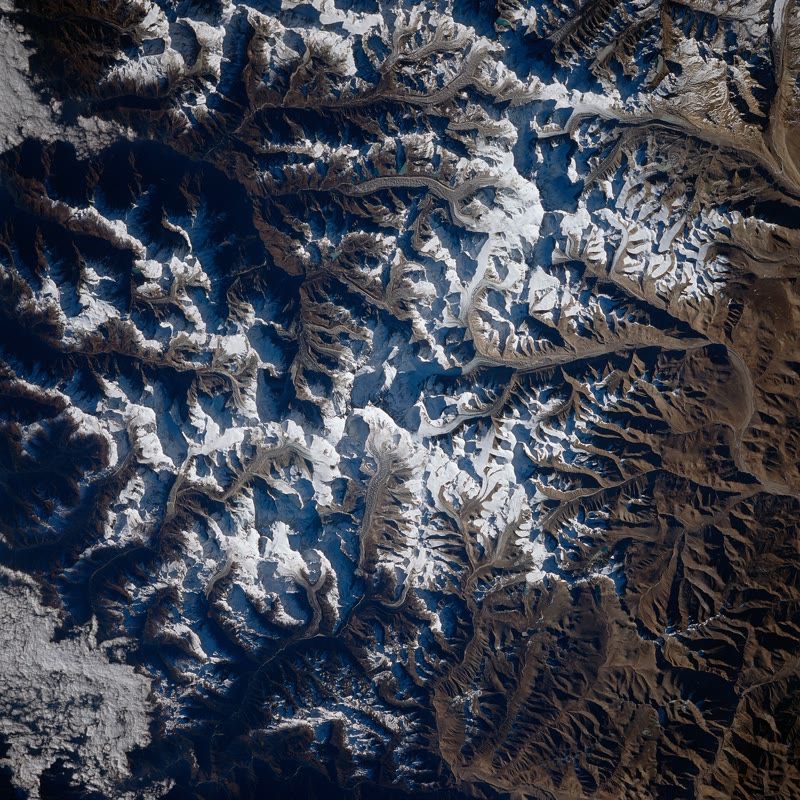
\includegraphics[width=0.5\linewidth]{images/book2/g12-nasa-everest-columbia.jpg}

{\small O monte Everest e muitas geleiras em volta dele, vistos do ônibus
espacial Columbia em 30 de novembro de 1996. Fotografia NASA (domínio
público).}
\end{omfigure}
% ledger: photo:g12-everest-columbia

\begin{recall}
Uma placa de \omterm{def:g11:ocean-ridges:oceanic-lithosphere}{litosfera oceânica}, formada numa dorsal, volta a afundar no
manto numa fossa; a sua \omterm{def:g11:subduction-zones:slab}{laje} a puxa para baixo
(\cref{ch:g11:subduction-zones}). A \omterm{def:g12:continental-crust:continental-crust}{crosta continental} é espessa e leve,
cerca de \qty{2830}{kg/m^3} em média contra \qty{3380}{kg/m^3} para o manto
abaixo dela, por isso ela flutua alto, e uma crosta espessa fica mais alta
que uma fina, sobre uma \omterm{def:g12:continental-crust:root}{raiz}
(\cref{ch:g12:continental-crust,ch:g11:lithosphere-asthenosphere}). Uma
falha é uma ruptura ao longo da qual os dois blocos se moveram; numa \omterm{def:g11:ocean-ridges:normal-fault}{falha
normal}, o bloco acima do plano de falha desceu, como onde a crosta é
estirada numa dorsal lenta (\cref{ch:g11:ocean-ridges}).
\end{recall}
% ledger: cm95:crust, data:prem, tulane:no-subduct, usgs:normal-fault

\section{Da subducção à colisão}

Um oceano que é consumido numa fossa mais depressa do que é produzido na sua
dorsal encolhe. Um continente levado pela placa que afunda se aproxima da
fossa à velocidade da placa, e acaba chegando a ela. A \omterm{def:g11:ocean-ridges:oceanic-lithosphere}{litosfera oceânica} à
sua frente já desceu; o continente não pode segui-la, porque a sua crosta é
leve demais para afundar no manto, mais denso. A \omterm{def:g11:subduction-zones:subduction}{subducção} para. Os dois
continentes são comprimidos um contra o outro, e a \omterm{def:g11:subduction-zones:slab}{laje} que pendia do fundo
oceânico acaba se rompendo e afundando no manto.
% ledger: earle:collision, tulane:no-subduct

\begin{definition}[Colisão continental]\label{def:g12:mountain-building:collision}
Uma \emph{colisão continental}\index{colisao continental@colisão continental} é o encontro de
dois continentes num limite de placas convergente, depois que a \omterm{def:g11:ocean-ridges:oceanic-lithosphere}{litosfera
oceânica} entre eles foi subductada. Nenhum dos continentes afunda: a crosta
entre eles é deformada e espessada num cinturão de montanhas.
\end{definition}
% ledger: earle:collision, tulane:no-subduct, usgs:himalaya-collision

\begin{omfigure}
\begin{tikzpicture}[x=0.95cm, y=0.95cm, font=\scriptsize]
  % ---- stage 1: the ocean closes ----
  \begin{scope}[yshift=0cm]
    \fill[omSea] (3.4,0) -- (8.6,0) -- (8.0,-0.5) -- (4.3,-0.5) -- (3.5,0.0) -- cycle;
    \fill[omLithGranite] (0,0.15) -- (3.5,0.15) -- (4.3,-0.5) -- (4.3,-0.75) -- (3.5,-1.0) -- (0,-1.0) -- cycle;
    \fill[omLithBasalt] (4.3,-0.5) -- (8.0,-0.5) .. controls (9.0,-0.75) and (9.6,-1.2) .. (10.4,-2.0)
      -- (10.15,-2.15) .. controls (9.4,-1.4) and (8.9,-1.0) .. (8.0,-0.75) -- (4.3,-0.75) -- cycle;
    \fill[omLithGranite] (8.0,-0.5) -- (8.6,0.2) -- (12,0.2) -- (12,-1.05) -- (9.5,-1.05)
      .. controls (9.0,-0.75) .. (8.0,-0.5) -- cycle;
    \fill[omThm!70] (10.0,0.2) -- (10.3,0.55) -- (10.6,0.2) -- cycle;
    \draw[black!60, line width=0.3pt] (0,0.15) -- (3.5,0.15) -- (4.3,-0.5) -- (8.0,-0.5) -- (8.6,0.2) -- (12,0.2);
    \draw[-{Stealth[length=2mm]}, line width=0.8pt] (1.2,0.45) -- (2.6,0.45);
    \node[anchor=east] at (0,-0.4) {1};
    \node at (1.8,-0.5) {continente};
    \node at (6.1,-0.25) {oceano};
    \node[anchor=north] at (6.1,-0.8) {litosfera oceânica};
    \node[anchor=south] at (8.0,0.0) {fossa};
    \node[anchor=south] at (10.3,0.55) {arco vulcânico};
    \node at (11.1,-0.5) {continente};
  \end{scope}
  % ---- stage 2: the continents meet ----
  \begin{scope}[yshift=-3.0cm]
    \fill[omSea] (6.9,0) -- (8.4,0) -- (8.0,-0.4) -- (7.4,-0.35) -- cycle;
    \fill[omLithGranite] (0,0.15) -- (6.8,0.15) -- (7.6,-0.4) -- (8.0,-0.5)
      .. controls (9.0,-0.75) .. (9.5,-1.05) -- (9.2,-1.4) -- (6.5,-1.0) -- (0,-1.0) -- cycle;
    \fill[omLithBasalt] (9.5,-1.05) .. controls (10.0,-1.4) .. (10.6,-2.0) -- (10.35,-2.15)
      .. controls (9.8,-1.6) .. (9.2,-1.4) -- cycle;
    \fill[omLithGranite] (8.0,-0.5) -- (8.6,0.2) -- (12,0.2) -- (12,-1.05) -- (9.5,-1.05)
      .. controls (9.0,-0.75) .. (8.0,-0.5) -- cycle;
    \fill[omLithPeridotite] (7.0,0.15) -- (7.9,0.15) -- (8.3,0.05) -- (7.95,-0.12) -- (7.3,0.0) -- cycle;
    \fill[omThm!70] (10.0,0.2) -- (10.3,0.55) -- (10.6,0.2) -- cycle;
    \draw[-{Stealth[length=2mm]}, line width=0.8pt] (3.2,0.45) -- (4.6,0.45);
    \node[anchor=east] at (0,-0.4) {2};
    \node at (3.4,-0.45) {continente};
    \draw[black!60] (7.6,0.12) -- (7.0,0.75) node[anchor=south east, inner sep=1pt] {lasca de fundo oceânico};
    \node at (11.1,-0.5) {continente};
    \node[anchor=west] at (10.7,-1.9) {laje};
  \end{scope}
  % ---- stage 3: a mountain belt ----
  \begin{scope}[yshift=-6.4cm]
    \fill[omLithGranite] (0,0.15) -- (4.5,0.15) .. controls (6.0,0.4) and (6.6,1.25) .. (7.6,1.3)
      .. controls (8.7,1.3) and (9.6,0.5) .. (10.6,0.2) -- (12,0.2) -- (12,-1.05) -- (10.6,-1.1)
      .. controls (9.5,-2.2) and (8.6,-2.6) .. (7.7,-2.6) .. controls (6.6,-2.6) and (5.6,-1.6) .. (4.5,-1.0)
      -- (0,-1.0) -- cycle;
    \draw[black!60, line width=0.3pt] (0,0.15) -- (4.5,0.15) .. controls (6.0,0.4) and (6.6,1.25) .. (7.6,1.3)
      .. controls (8.7,1.3) and (9.6,0.5) .. (10.6,0.2) -- (12,0.2);
    \draw[black!60, dashed, line width=0.4pt] (0,-1.0) -- (4.5,-1.0) .. controls (5.6,-1.6) and (6.6,-2.6) .. (7.7,-2.6)
      .. controls (8.6,-2.6) and (9.5,-2.2) .. (10.6,-1.1) -- (12,-1.05);
    \draw[omThm, line width=1.0pt] (7.0,1.25) -- (8.3,-2.55);
    \foreach \t in {0.15,0.4,0.65}
      \fill[omLithPeridotite] ($(7.0,1.25)!\t!(8.3,-2.55)$) ++(-0.12,0.05) -- ++(0.3,0) -- ++(-0.05,-0.22) -- ++(-0.3,0) -- cycle;
    \fill[omLithBasalt] (10.9,-1.9) -- (11.5,-2.35) -- (11.35,-2.5) -- (10.75,-2.05) -- cycle;
    \node[anchor=east] at (0,-0.4) {3};
    \node at (2.4,-0.45) {continente};
    \node at (11.3,-0.5) {continente};
    \draw[black!60] (7.2,0.6) -- (5.9,1.5) node[anchor=east, inner sep=1pt] {sutura com ofiolitos};
    \node at (7.7,-1.9) {raiz};
    \node[anchor=north] at (11.2,-2.5) {laje rompida};
    \node[anchor=south] at (7.6,1.35) {\shortstack{cinturão de\\montanhas}};
  \end{scope}
\end{tikzpicture}

{\small Da \omterm{def:g11:subduction-zones:subduction}{subducção} à colisão (fora de escala). 1: um oceano se fecha à
medida que o seu fundo afunda numa fossa. 2: o continente chega à fossa e não
pode afundar; lascas de fundo oceânico são empurradas sobre a sua borda.
3: a crosta entre os dois continentes é encurtada e espessada num cinturão
de montanhas que fica sobre uma \omterm{def:g12:continental-crust:root}{raiz}; a linha onde os dois continentes se
juntam, marcada por lascas de fundo oceânico, é a \omterm{def:g12:mountain-building:suture}{sutura}; a \omterm{def:g11:subduction-zones:slab}{laje} se rompe e
afunda.}
\end{omfigure}
% ledger: earle:collision, tulane:ocean-basins, usgs:suture, tulane:roots

\subsection{O vestígio de um oceano desaparecido}

Quando o oceano se fechou, os dois continentes ficam soldados ao longo de
uma linha.

\begin{definition}[Sutura]\label{def:g12:mountain-building:suture}
Uma \emph{sutura}\index{sutura} é a linha, ou a zona estreita, ao longo da
qual dois continentes foram unidos por uma colisão, depois que a \omterm{def:g11:subduction-zones:subduction}{subducção}
entre eles parou: o vestígio de um antigo limite de placas. Ela marca onde
ficava o oceano entre eles.
\end{definition}
% ledger: usgs:suture, liu20:itsz

O que marca uma \omterm{def:g12:mountain-building:suture}{sutura}? Ao longo de muitas delas há corpos de rocha que não
pertencem a nenhum lugar de um continente: de cima para baixo, sedimentos
marinhos, basaltos em almofada, uma massa de \omterm{def:g11:igneous-rocks:intrusion}{diques} verticais lado a lado,
\omterm{def:g11:ocean-ridges:gabbro}{gabro} e, na base, \omterm{def:g11:ocean-ridges:peridotite}{peridotito} do manto: as camadas do fundo oceânico
(\cref{ch:g11:ocean-ridges}), com o topo do manto abaixo delas.
% ledger: tulane:ocean-basins

\begin{definition}[Ofiolito]\label{def:g12:mountain-building:ophiolite}
Um \emph{ofiolito}\index{ofiolito} é um pedaço de \omterm{def:g11:ocean-ridges:oceanic-lithosphere}{litosfera oceânica} ---
sedimentos, basaltos em almofada, complexo de \omterm{def:g11:igneous-rocks:intrusion}{diques}, \omterm{def:g11:ocean-ridges:gabbro}{gabro} e \omterm{def:g11:ocean-ridges:peridotite}{peridotito} do
manto --- empurrado sobre a \omterm{def:g12:continental-crust:continental-crust}{crosta continental}.
\end{definition}
% ledger: tulane:ocean-basins

Um \omterm{def:g12:mountain-building:ophiolite}{ofiolito} é fundo oceânico encalhado: uma lasca do oceano desaparecido,
empurrada sobre um continente em vez de afundar com o resto. As montanhas
erguidas por uma colisão contêm comumente um pouco de \omterm{def:g11:ocean-ridges:oceanic-lithosphere}{crosta oceânica} e de
manto superior, porque é ali que um oceano se fechou. No sul do Tibete, os
\omterm{def:g12:mountain-building:ophiolite}{ofiolitos} alinhados ao longo da \omterm{def:g12:mountain-building:suture}{sutura} do Indo--Tsangpo são restos de um
oceano chamado Neotétis, que ficava entre a Índia e a região de Lhasa; um
\omterm{def:g11:ocean-ridges:gabbro}{gabro} dali foi datado de 243 milhões de anos.
% ledger: tulane:ocean-basins, earle:collision, liu20:itsz

\begin{omfigure}
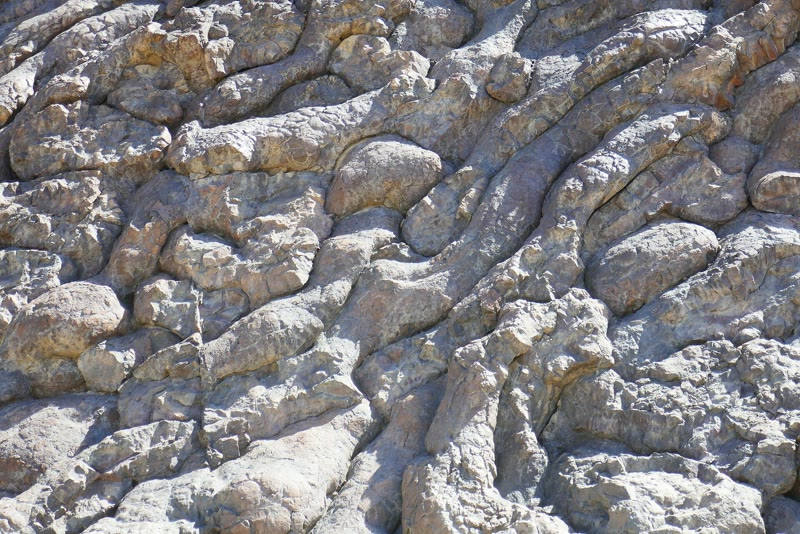
\includegraphics[width=0.6\linewidth]{images/book2/g12-duchoiselle-oman-pillows.jpg}

{\small Lavas em almofada do \omterm{def:g12:mountain-building:ophiolite}{ofiolito} de Semail em Wadi Jizzi, Omã: lava que
esfriou debaixo d'água em almofadas arredondadas, hoje em terra firme.
Fotografia Lionel Duchoiselle (CC~BY-SA~3.0).}
\end{omfigure}
% ledger: photo:g12-oman-pillows

\section{Encurtar a crosta}

Comprimido pelos lados, um corpo de rocha se rompe se está frio e frágil; se
está quente o bastante para se comportar de modo plástico, ele se dobra. Um
cinturão de montanhas está cheio de \omterm{def:g12:mountain-building:fold}{dobras} e de falhas.
% ledger: earle:folds

\subsection{As dobras}

\begin{definition}[Dobra; anticlinal; sinclinal; eixo de dobra]\label{def:g12:mountain-building:fold}
Uma \emph{dobra}\index{dobra} é uma curvatura em camadas de rocha. Os seus
lados inclinados são os \emph{flancos}; eles se encontram na
\emph{charneira}, onde as camadas são mais curvas, e a linha ao longo da
charneira é o \emph{eixo de dobra}\index{eixo de dobra}. Um
\emph{anticlinal}\index{anticlinal} é uma dobra cujas camadas se curvam
para cima, com os flancos mergulhando para longe do eixo; um
\emph{sinclinal}\index{sinclinal} é uma dobra cujas camadas se curvam para
baixo, com os flancos mergulhando em direção ao eixo.
\end{definition}
% ledger: earle:folds, tulane:fold-geometry

O plano que passa pelas charneiras das camadas sucessivas é o plano axial.
\omterm{def:g12:mountain-building:fold}{Anticlinais} e \omterm{def:g12:mountain-building:fold}{sinclinais} costumam vir aos pares, o flanco de um sendo o
flanco do seguinte. As \omterm{def:g12:mountain-building:fold}{dobras} têm todos os tamanhos, do microscópico a
dezenas de quilômetros de largura. Uma vez erodido, um \omterm{def:g12:mountain-building:fold}{anticlinal} mostra as
suas camadas mais antigas no núcleo e um \omterm{def:g12:mountain-building:fold}{sinclinal} as mais jovens; um
\omterm{def:g12:mountain-building:fold}{anticlinal} não é necessariamente uma crista, nem um \omterm{def:g12:mountain-building:fold}{sinclinal} um vale,
porque a erosão segue as camadas duras e moles, e não a forma da \omterm{def:g12:mountain-building:fold}{dobra}.
% ledger: earle:folds, tulane:fold-geometry

\begin{omfigure}
\begin{tikzpicture}[x=1.2cm, y=1.2cm, font=\scriptsize]
  \def\W{6}\def\H{2.0}\def\dx{1.35}\def\dy{0.78}
  \tikzset{declare function={zb(\x,\c)=\c+0.8*cos(60*(\x-1.5));}}
  \colorlet{bandA}{omLithSchist!70}\colorlet{bandB}{omLithSand}\colorlet{bandC}{omLithShale}
  \colorlet{bandD}{icsJurassic!35}\colorlet{bandE}{icsTriassic!35}\colorlet{bandF}{icsCretaceous!45}
  % front face
  \begin{scope}
    \clip (0,0) rectangle (\W,\H);
    \fill[bandA] (0,0) rectangle (\W,\H);
    \foreach \c/\col in {0.0/bandB, 0.6/bandC, 1.2/bandD, 1.8/bandE, 2.4/bandF}
      \fill[\col] plot[domain=0:\W, samples=80, smooth] (\x,{zb(\x,\c)}) -- (\W,4) -- (0,4) -- cycle;
    \foreach \c in {0.0,0.6,1.2,1.8,2.4}
      \draw[black!55, line width=0.35pt] plot[domain=0:\W, samples=80, smooth] (\x,{zb(\x,\c)});
  \end{scope}
  % top face: outcrop bands (crossings of the top surface computed for these curves)
  \fill[bandE] (0,\H) -- (0.242,\H) -- ++(\dx,\dy) -- (\dx,\H+\dy) -- cycle;
  \fill[bandD] (0.242,\H) -- (2.758,\H) -- ++(\dx,\dy) -- (0.242+\dx,\H+\dy) -- cycle;
  \fill[bandE] (2.758,\H) -- (3.5,\H) -- ++(\dx,\dy) -- (2.758+\dx,\H+\dy) -- cycle;
  \fill[bandF] (3.5,\H) -- (5.5,\H) -- ++(\dx,\dy) -- (3.5+\dx,\H+\dy) -- cycle;
  \fill[bandE] (5.5,\H) -- (\W,\H) -- ++(\dx,\dy) -- (5.5+\dx,\H+\dy) -- cycle;
  \foreach \x in {0.242,2.758,3.5,5.5} \draw[black!55, line width=0.35pt] (\x,\H) -- ++(\dx,\dy);
  % right face: the layers meet it at constant heights (cylindrical folds)
  \foreach \lo/\hi/\col in {0.0/0.6/bandB, 0.6/1.2/bandC, 1.2/1.8/bandD, 1.8/2.0/bandE}
    \fill[\col] (\W,\lo) -- (\W+\dx,\lo+\dy) -- (\W+\dx,\hi+\dy) -- (\W,\hi) -- cycle;
  \foreach \y in {0.6,1.2,1.8} \draw[black!55, line width=0.35pt] (\W,\y) -- ++(\dx,\dy);
  % outline
  \draw[black, line width=0.5pt] (0,0) rectangle (\W,\H) (0,\H) -- (\dx,\H+\dy) -- (\W+\dx,\H+\dy) -- (\W,\H)
    (\W+\dx,\H+\dy) -- (\W+\dx,\dy) -- (\W,0);
  % fold axes on the top face, axial planes on the front face
  \draw[omThm, line width=1pt] (1.5,\H) -- ++(\dx,\dy);
  \draw[omDef, line width=1pt] (4.5,\H) -- ++(\dx,\dy);
  \draw[omThm, dashed, line width=0.6pt] (1.5,0) -- (1.5,\H);
  \draw[omDef, dashed, line width=0.6pt] (4.5,0) -- (4.5,\H);
  \node[anchor=south, omThm] at (1.5+\dx,\H+\dy) {anticlinal: eixo de dobra};
  \node[anchor=south, omDef] at (4.5+\dx,\H+\dy) {sinclinal: eixo de dobra};
  \draw[black!70] (3.2,0.95) -- (3.9,-0.35) node[anchor=north] {flanco};
  \draw[black!70] (1.5,1.4) circle (0.07) -- (0.4,-0.35) node[anchor=north] {charneira};
  \draw[black!70] (1.5,0.25) -- (2.0,-0.35) node[anchor=north] {plano axial};
\end{tikzpicture}

{\small Um \omterm{def:g12:mountain-building:fold}{anticlinal} e um \omterm{def:g12:mountain-building:fold}{sinclinal}, cortados por uma superfície plana de
erosão (bloco-diagrama, fora de escala). Os \omterm{def:g12:mountain-building:fold}{eixos de dobra} correm ao longo
das charneiras; as linhas tracejadas são os traços dos planos axiais. Na
superfície de cima, o \omterm{def:g12:mountain-building:fold}{anticlinal} erodido mostra camadas mais antigas no seu
núcleo, o \omterm{def:g12:mountain-building:fold}{sinclinal} camadas mais jovens.}
\end{omfigure}
% ledger: earle:folds, tulane:fold-geometry

\begin{omfigure}
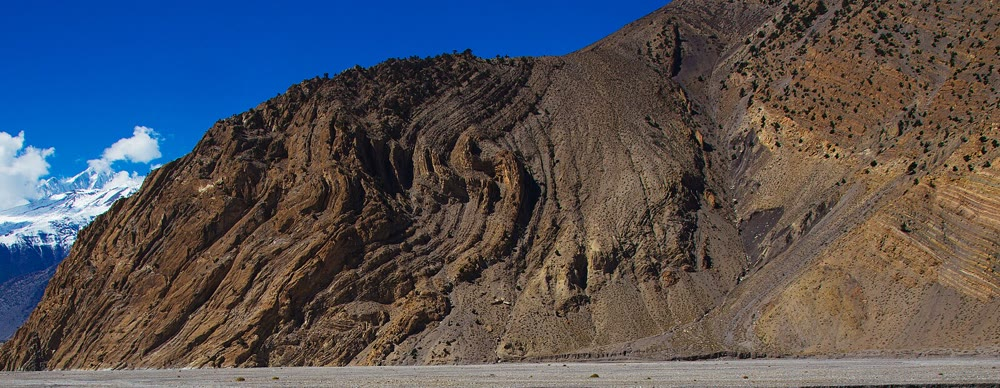
\includegraphics[width=0.95\linewidth]{images/book2/g12-hullot-kali-gandaki-folds.jpg}

{\small Camadas de rocha dobradas num paredão do Himalaia, cerca de
\qty{3}{km} a nordeste de Jomsom, na garganta do Kali Gandaki, no Nepal.
Fotografia Jean-Marie Hullot (CC~BY~2.0).}
\end{omfigure}
% ledger: photo:g12-kali-gandaki

A cobertura das Colinas de Varden está dobrada da mesma maneira, muito mais
suavemente. O seu arenito, o seu calcário, o seu folhelho e o seu giz foram
depositados na horizontal, e depois curvados num \omterm{def:g12:mountain-building:fold}{anticlinal} e num \omterm{def:g12:mountain-building:fold}{sinclinal}
cujos flancos mergulham \ang{12}; uma \omterm{def:g11:ocean-ridges:normal-fault}{falha normal} posterior os corta.
% ledger: region:name; model in figdata/shared/region.py (LIMB_DIP 12, AXIS_ANTI 3.5 km, AXIS_SYN 7.5 km)

\begin{omfigure}
\begin{tikzpicture}
\begin{axis}[omsection, x=1.25cm, y=0.003125cm, xmin=0, xmax=9.49, ymin=-700, ymax=650,
  xlabel={distância a partir de A (\unit{km})}, ylabel={altitude (\unit{m})},
  ytick={-600,-300,0,300,600}, tick label style={font=\scriptsize}]
\addplot[fill=black!8, draw=black!50, line width=0.3pt, even odd rule] table {figdata/out/shared-region-section-unit-schist.dat};
\addplot[fill=icsTriassic!20, draw=black!50, line width=0.3pt, even odd rule] table {figdata/out/shared-region-section-unit-sandstone.dat};
\addplot[fill=icsJurassic!25, draw=black!50, line width=0.3pt, even odd rule] table {figdata/out/shared-region-section-unit-limestone.dat};
\addplot[fill=icsJurassic!8, draw=black!50, line width=0.3pt, even odd rule] table {figdata/out/shared-region-section-unit-shale.dat};
\addplot[fill=icsCretaceous!20, draw=black!50, line width=0.3pt, even odd rule] table {figdata/out/shared-region-section-unit-chalk.dat};
\addplot[fill=omLithAlluv, draw=black!50, line width=0.3pt, even odd rule] table {figdata/out/shared-region-section-unit-alluvium.dat};
\addplot[black, line width=0.7pt] table {figdata/out/shared-region-section-ground.dat};
\addplot[fault] table {figdata/out/shared-region-section-fault.dat};
% axis positions from figdata/grade-12/fold_shortening.py (section_anticline_km, section_syncline_km; the syncline lies on the hanging wall, shifted by the fault heave)
\draw[omThm, dashed, line width=0.7pt] (axis cs:3.162,-700) -- (axis cs:3.162,660);
\draw[omDef, dashed, line width=0.7pt] (axis cs:7.484,-700) -- (axis cs:7.484,660);
\node[anchor=south, omThm, font=\scriptsize] at (axis cs:3.162,660) {eixo do anticlinal};
\node[anchor=south, omDef, font=\scriptsize] at (axis cs:7.484,660) {eixo do sinclinal};
\node[anchor=south east, font=\small\bfseries] at (axis cs:0,650) {A};
\node[anchor=south west, font=\small\bfseries] at (axis cs:9.49,650) {B};
\node[font=\scriptsize, fill=white, inner sep=1pt] at (axis cs:1.2,-520) {xisto};
\node[font=\scriptsize, fill=white, inner sep=1pt, anchor=east] at (axis cs:6.55,-450) {falha normal};
\end{axis}
\end{tikzpicture}

\smallskip
{\small\tikz\fill[black!8, draw=black!50] (0,0) rectangle (0.35,0.22);~xisto \quad
\tikz\fill[icsTriassic!20, draw=black!50] (0,0) rectangle (0.35,0.22);~arenito \quad
\tikz\fill[icsJurassic!25, draw=black!50] (0,0) rectangle (0.35,0.22);~calcário \quad
\tikz\fill[icsJurassic!8, draw=black!50] (0,0) rectangle (0.35,0.22);~folhelho \quad
\tikz\fill[icsCretaceous!20, draw=black!50] (0,0) rectangle (0.35,0.22);~giz \quad
\omve{2.5}}

{\small Corte A--B através das Colinas de Varden, de sudoeste para nordeste.
A cobertura assenta sobre o embasamento de xisto e está dobrada num
\omterm{def:g12:mountain-building:fold}{anticlinal} e num \omterm{def:g12:mountain-building:fold}{sinclinal}; a \omterm{def:g11:ocean-ridges:normal-fault}{falha normal}, mais jovem que as \omterm{def:g12:mountain-building:fold}{dobras}, faz
descer o bloco do nordeste. A escala vertical está esticada 2.5 vezes, o
que faz os flancos parecerem mais íngremes do que são. Dados: o modelo da
região usado nesta série.}
\end{omfigure}
% ledger: region:name; computed in figdata/shared/region.py (section A-B)

\subsection{Falhas inversas, cavalgamentos e nappes}

Onde a crosta é comprimida enquanto está fria e frágil, ela se rompe ao
longo de falhas de outro tipo que as \omterm{def:g11:ocean-ridges:normal-fault}{falhas normais} da crosta estirada.

\begin{definition}[Falha inversa; cavalgamento]\label{def:g12:mountain-building:thrust}
Uma \emph{falha inversa}\index{falha inversa} é uma falha inclinada ao longo
da qual o bloco acima do plano de falha subiu em relação ao bloco abaixo
dele. As falhas inversas se formam onde a crosta é comprimida. Um
\emph{cavalgamento}\index{cavalgamento} é uma falha inversa de mergulho
suave, menor que \ang{45}.
\end{definition}
% ledger: earle:reverse-thrust, tulane:fold-geometry

Um \omterm{def:g12:mountain-building:thrust}{cavalgamento} pode levar uma lâmina de rocha por dezenas de quilômetros,
e então rochas mais antigas vêm repousar sobre rochas mais jovens, contra a
ordem em que foram depositadas. Nas Montanhas Rochosas, o cavalgamento de
McConnell empurrou uma pilha de rochas sedimentares de cerca de
\qty{800}{m} de espessura por uns \qty{40}{km} de oeste para leste: um
calcário de cerca de 500 milhões de anos repousa hoje sobre um lamito de
cerca de 75 milhões de anos.
% ledger: earle:reverse-thrust

\begin{definition}[Nappe]\label{def:g12:mountain-building:nappe}
Uma \emph{nappe}\index{nappe} é uma grande lâmina de rocha que foi levada
por uma longa distância, muitas vezes dezenas de quilômetros, por cima das
rochas abaixo dela, ao longo de um \omterm{def:g12:mountain-building:thrust}{cavalgamento} quase horizontal.
\end{definition}
% ledger: ngu:nappe, earle:reverse-thrust

Uma \omterm{def:g12:mountain-building:nappe}{nappe} pode levar rochas formadas longe dali, até lascas de fundo
oceânico; ela mesma pode ser dobrada, com as suas camadas invertidas. Os
cinturões de montanhas empilham \omterm{def:g12:mountain-building:nappe}{nappes} umas sobre as outras. Mais tarde, a
erosão abre buracos através de uma \omterm{def:g12:mountain-building:nappe}{nappe}, abrindo janelas para as rochas de
baixo, e deixa pedaços isolados dela sobre as rochas mais jovens.
% ledger: ngu:nappe

\begin{omfigure}
\begin{tikzpicture}[x=1.0cm, y=1.0cm, font=\scriptsize]
  % rocks in place (younger), flat-lying
  \fill[icsCretaceous!25] (0,-1.6) rectangle (12,-0.4);
  \fill[icsJurassic!25] (0,-1.6) rectangle (12,-1.1);
  \draw[black!50, line width=0.3pt] (0,-1.1) -- (12,-1.1);
  \fill[white] (5.6,-0.4) -- (6.2,-0.62) -- (6.8,-0.4) -- cycle;
  % the nappe (older rocks) above a nearly flat thrust, cut by erosion
  \fill[omLithSchist!80] (0.8,-0.4) .. controls (1.2,0.35) and (1.9,0.35) .. (2.3,-0.4) -- cycle;
  \fill[omLithSchist!80] (3.2,-0.4) .. controls (3.9,0.9) and (4.8,0.9) .. (5.6,-0.4) -- cycle;
  \fill[omLithSchist!80] (6.8,-0.4) .. controls (7.1,0.9) and (7.7,1.3) .. (8.4,1.25) -- (12,0.9) -- (12,-0.4) -- cycle;
  % ground surface
  \draw[black, line width=0.6pt] (0,-0.4) -- (0.8,-0.4) .. controls (1.2,0.35) and (1.9,0.35) .. (2.3,-0.4)
     -- (3.2,-0.4) .. controls (3.9,0.9) and (4.8,0.9) .. (5.6,-0.4) -- (6.2,-0.62) -- (6.8,-0.4)
     .. controls (7.1,0.9) and (7.7,1.3) .. (8.4,1.25) -- (12,0.9);
  % thrust traces (teeth on the block that moved over)
  \draw[thrust fault] (0.8,-0.4) -- (2.3,-0.4);
  \draw[thrust fault] (3.2,-0.4) -- (5.6,-0.4);
  \draw[thrust fault] (6.8,-0.4) -- (12,-0.4);
  \draw[-{Stealth[length=2mm]}, line width=0.9pt] (11.4,1.45) -- (9.6,1.6);
  \node[anchor=south] at (10.5,1.55) {movimento da nappe};
  \node at (9.9,0.3) {nappe: rochas mais antigas};
  \node[fill=white, inner sep=1pt] at (2.0,-0.85) {rochas no lugar: mais jovens};
  \draw[black!60] (1.55,0.0) -- (1.3,0.8) node[anchor=south] {pedaço isolado};
  \draw[black!60] (6.2,-0.58) -- (6.2,-0.68) node[anchor=north, fill=white, inner sep=1pt] {janela};
  \draw[black!60] (9.0,-0.42) -- (9.3,-0.68) node[anchor=north, fill=white, inner sep=1pt] {cavalgamento};
\end{tikzpicture}

{\small Uma \omterm{def:g12:mountain-building:nappe}{nappe} (fora de escala): uma lâmina de rochas mais antigas levada
ao longo de um \omterm{def:g12:mountain-building:thrust}{cavalgamento} quase horizontal sobre rochas mais jovens que
ficaram no lugar. A erosão abriu uma janela através dela e deixou um pedaço
isolado dela à esquerda. Os dentes sobre o \omterm{def:g12:mountain-building:thrust}{cavalgamento} apontam para o bloco
que se moveu por cima.}
\end{omfigure}
% ledger: ngu:nappe, earle:reverse-thrust

\begin{omfigure}
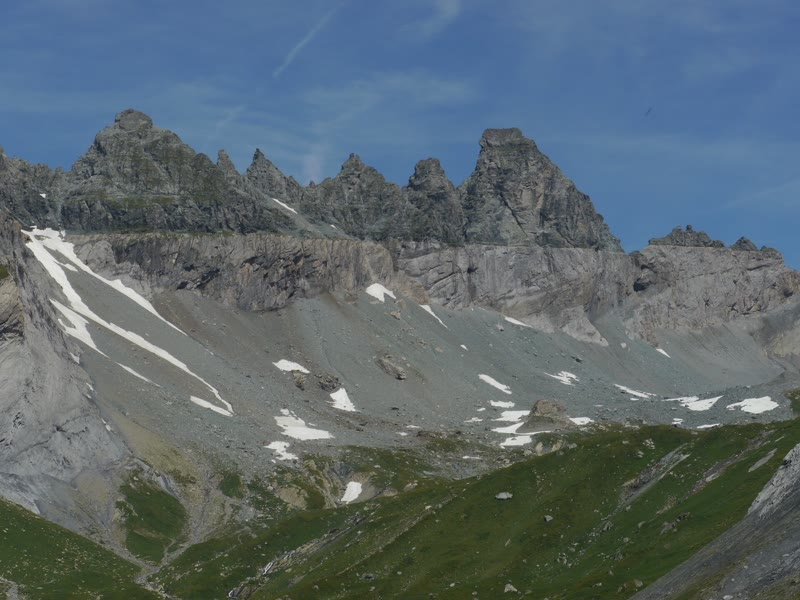
\includegraphics[width=0.5\linewidth]{images/book2/g12-heine-glarus-thrust.jpg}

{\small O cavalgamento de Glarus, nos Alpes do leste da Suíça. As rochas
escuras dos picos, depositadas no Permiano, entre cerca de 299 e 252 milhões
de anos atrás, repousam sobre rochas mais claras e muito mais jovens; o
\omterm{def:g12:mountain-building:thrust}{cavalgamento} é o limite nítido entre elas. As rochas de cima se deslocaram
uns 40 a \qty{50}{km}. Fotografia Christian Heine (CC~BY-SA~3.0).}
\end{omfigure}
% ledger: photo:g12-glarus (Verrucano, Permian; displacement 40-50 km, Pfiffner 1985), ics:base.Permian, ics:base.Triassic

\subsection{Medir o encurtamento}

As \omterm{def:g12:mountain-building:fold}{dobras} e os \omterm{def:g12:mountain-building:thrust}{cavalgamentos} tornam a crosta mais curta na direção em que
ela é comprimida.

\begin{definition}[Encurtamento]\label{def:g12:mountain-building:shortening}
O \emph{encurtamento}\index{encurtamento} de uma camada é a fração do seu
comprimento que ela perdeu: se ela media $L_0$ e hoje se estende por $L$,
\[
  e = \frac{L_0 - L}{L_0}.
\]
\end{definition}

Para medi-lo, é preciso o comprimento original $L_0$. Em muitas \omterm{def:g12:mountain-building:fold}{dobras}, as
camadas conservam a sua espessura ao se curvar, deslizando umas sobre as
outras como as páginas de um livro dobrado; uma camada assim não é esticada
ao longo do seu comprimento. Isso dá o comprimento original.
% ledger: tulane:fold-geometry (flexural folds keep their thickness)

\begin{proposition}[O encurtamento de uma camada dobrada]\label{prop:g12:mountain-building:shortening}
Se uma camada se dobrou sem ser esticada nem comprimida ao longo de si
mesma, o seu comprimento original $L_0$ é o seu comprimento medido ao longo
da camada dobrada. Para uma \omterm{def:g12:mountain-building:fold}{dobra} de flancos retos que mergulham com um
ângulo $\theta$,
\[
  e = 1 - \cos\theta .
\]
\end{proposition}

\begin{proof}
Desdobrar a camada, sem esticá-la, a estende na horizontal com o seu
comprimento inalterado; logo $L_0$ é o comprimento ao longo da camada. Num
flanco reto de comprimento $\ell$ que mergulha com $\theta$, a distância
horizontal coberta é $\ell\cos\theta$ (triângulo retângulo). Somando todos os
flancos, a camada de comprimento $L_0$ se estende por $L = L_0\cos\theta$, e
$e = (L_0 - L_0\cos\theta)/L_0 =
1 - \cos\theta$.
\end{proof}

\begin{omfigure}
\begin{tikzpicture}
\begin{axis}[name=sine, x=2.0cm, y=2.0cm, axis lines=none,
  xmin=-0.05, xmax=2.25, ymin=-0.4, ymax=0.8, clip=false]
% computed in figdata/grade-12/fold_shortening.py (part sine: A/lambda = 0.25, e = 31.7 %)
\addplot[omLithSand!80!black, line width=1.6pt] table[x=x, y=y] {figdata/out/grade-12-fold_shortening-sine.dat};
\draw[omThm, line width=1.6pt] (axis cs:0,0.62) -- (axis cs:2.196,0.62);
\draw[black!60, |-|] (axis cs:0,-0.32) -- node[below, font=\scriptsize] {$L$ (hoje)} (axis cs:1.5,-0.32);
\node[anchor=south west, font=\scriptsize, omThm] at (axis cs:0,0.64) {$L_0$: a mesma camada desdobrada};
\end{axis}
\begin{axis}[omrecord, at={(sine.east)}, anchor=west, xshift=1.4cm, width=0.46\linewidth, height=4.6cm,
  xmin=0, xmax=80, ymin=0, ymax=85, xlabel={mergulho dos flancos $\theta$ (\unit{\degree})},
  ylabel={encurtamento $e$ (\unit{\percent})}, xtick={0,20,...,80}]
% computed in figdata/grade-12/fold_shortening.py (part dip: e = 1 - cos theta)
\addplot[omProp, line width=1pt] table[x=theta, y=e_pct] {figdata/out/grade-12-fold_shortening-dip.dat};
\addplot[only marks, mark=*, mark size=1.6pt, omThm] coordinates {(12,2.185) (30,13.397) (60,50)};
\node[anchor=south, font=\scriptsize, align=center] at (axis cs:12,6) {Varden:\\\qty{2.2}{\percent}};
\node[anchor=west, font=\scriptsize] at (axis cs:32,10) {\qty{13}{\percent}};
\node[anchor=south east, font=\scriptsize] at (axis cs:60,51) {\qty{50}{\percent}};
\end{axis}
\end{tikzpicture}

{\small À esquerda: uma camada dobrada se estende por $L$; estendida na
horizontal, sem ser esticada, ela mede $L_0$ (aqui as \omterm{def:g12:mountain-building:fold}{dobras} são tão altas
quanto um quarto do seu comprimento de onda, e $L$ é \qty{68}{\percent} de
$L_0$). À direita: o \omterm{def:g12:mountain-building:shortening}{encurtamento} de uma \omterm{def:g12:mountain-building:fold}{dobra} de flancos retos,
$1 - \cos\theta$, em função do mergulho dos seus flancos. As \omterm{def:g12:mountain-building:fold}{dobras} suaves
encurtam muito pouco uma camada.}
\end{omfigure}
% values: sine_025_e_pct 31.68 (L/L0 = 0.683); varden_e_pct 2.1852; chevron_30 13.397; chevron_60 50 (fold_shortening.py)

\begin{method}[Medir o encurtamento num corte]\label{met:g12:mountain-building:shortening}
\begin{enumerate}
  \item Verifique se o corte está desenhado em escala verdadeira. Se a sua
        escala vertical está esticada, os mergulhos e os comprimentos ao
        longo das camadas são grandes demais: redesenhe-o, ou corrija
        primeiro cada mergulho.
  \item Escolha um limite de camada que possa ser seguido através do corte;
        onde uma falha o corta, junte as duas extremidades cortadas como
        estavam antes de a falha se mover.
  \item Meça o seu comprimento ao longo da camada, $L_0$: siga-o com um fio,
        ou some pequenos trechos retos.
  \item Meça a distância horizontal entre as suas duas extremidades, $L$.
  \item Calcule $e = (L_0 - L)/L_0$; para flancos retos de mergulho
        conhecido, $e = 1 - \cos\theta$ o dá de imediato.
\end{enumerate}
\end{method}

\begin{example}[As dobras de Varden]\label{ex:g12:mountain-building:varden}
Os flancos das \omterm{def:g12:mountain-building:fold}{dobras} de Varden mergulham \ang{12}, logo a cobertura foi
encurtada de $e = 1 - \cos\ang{12} = 1 - 0.978 = 0.022$, cerca de
\qty{2.2}{\percent}: uma faixa da região que hoje tem \qty{10}{km} de largura
tinha $10/\cos\ang{12} \approx
\qty{10.22}{km}$ de largura antes do dobramento. Medidos no corte A--B tal como está desenhado, os flancos
pareceriam ter cerca de \ang{28} de mergulho, porque a escala vertical está
esticada 2.5 vezes: $\tan\theta$ é multiplicada por 2.5, e $\arctan(2.5
\tan\ang{12}) \approx \ang{28}$. Lido ao pé da letra, isso daria um
\omterm{def:g12:mountain-building:shortening}{encurtamento} de \qty{12}{\percent}, mais de cinco vezes demais.
\end{example}
% values: varden_e_pct 2.1852, varden_L0_for_10km 10.223 (fold_shortening.py); arctan(2.5 x 0.2126) = 27.98 deg; 1 - cos 27.98 = 0.117

As \omterm{def:g12:mountain-building:fold}{dobras} suaves absorvem pouco. Um cinturão fortemente dobrado, com flancos
que mergulham \ang{60}, foi encurtado pela metade; e um único \omterm{def:g12:mountain-building:thrust}{cavalgamento}
quase horizontal que levou uma \omterm{def:g12:mountain-building:nappe}{nappe} por \qty{40}{km} absorve \qty{40}{km}
de \omterm{def:g12:mountain-building:shortening}{encurtamento}, tanto quanto um cinturão muito largo de \omterm{def:g12:mountain-building:fold}{dobras} suaves.

\section{Espessamento e soerguimento}

O \omterm{def:g12:mountain-building:shortening}{encurtamento} não destrói rocha. Uma faixa de crosta comprimida a uma
fração da sua largura anterior conserva o seu volume, então ela precisa
ficar mais espessa: se uma crosta de espessura $H_0$ é encurtada de uma
largura $L_0$ para $L$ ao longo de todo o comprimento do cinturão, a sua
seção conserva a sua área, $H L = H_0 L_0$, e
\[
  H = H_0\,\frac{L_0}{L} = \frac{H_0}{1 - e}.
\]
Uma crosta de \qty{35}{km} de espessura encurtada em \qty{50}{\percent}
passa a ter \qty{70}{km} de espessura. Depois, a \omterm{def:g11:lithosphere-asthenosphere:isostasy}{isostasia} faz o resto: uma
crosta mais espessa flutua mais alto, sobre uma \omterm{def:g12:continental-crust:root}{raiz} mais profunda
(\cref{prop:g11:lithosphere-asthenosphere:airy}). Com o modelo de Airy e as
densidades do lembrete, uma crosta mais espessa de $\Delta H$ fica mais alta
de $\Delta H\,(\rho_m - \rho_c)/\rho_m = \Delta H
\times 550/3380$, cerca de um sexto da espessura a mais; os outros cinco
sextos formam a \omterm{def:g12:continental-crust:root}{raiz}. A crosta tem de \num{35} a \qty{40}{km} de espessura
longe dos cinturões de montanhas, e de 50 a \qty{70}{km} sob eles: quanto
mais altas as montanhas, mais espessa a crosta.
% ledger: tulane:roots, cm95:crust, data:prem

Foi assim que o calcário do fundo do mar chegou ao topo do Everest:
depositado no fundo de um mar, ele foi levado para o norte com a Índia,
empilhado nas lâminas de \omterm{def:g12:mountain-building:thrust}{cavalgamento} do Himalaia e erguido à medida que a
crosta abaixo dele se espessava e subia. Esse movimento vertical da crosta
se chama soerguimento.
% ledger: sakai05:summit, sakai05:stacking, tulane:roots (uplift), usgs:himalaya-collision

\section{Duas cadeias}

\subsection{O Himalaia}

O Himalaia se estende por \qty{2900}{km} ao longo da fronteira entre a Índia
e o Tibete. Há cerca de 80 milhões de anos, a Índia ficava a cerca de
\qty{6400}{km} ao sul da Ásia, do outro lado de um oceano, e se movia para o
norte a cerca de \qty{9}{cm} por ano; ela encontrou a Ásia entre 40 e 50
milhões de anos atrás, e o seu avanço para o norte então diminuiu. As
reconstruções de placas mostram a viagem em detalhe: construídas a partir
de muitos tipos de evidência, entre eles os \omterm{def:g11:plate-motions:hotspot-track}{rastros de pontos quentes}
(\cref{ch:g11:plate-motions}), elas levam as placas de volta no tempo, passo
a passo.
% ledger: usgs:himalaya-collision, muller19:frame, muller22:frame

\begin{omfigure}
\begin{tikzpicture}
\begin{axis}[omrecord, omage, name=lat, width=0.5\linewidth, height=5.2cm,
  xmin=0, xmax=100, ymin=-45, ymax=35, xlabel={idade (\unit{Ma})}, ylabel={latitude (\unit{\degree})},
  xtick={0,20,...,100}, ytick={-40,-20,...,40},
  legend style={font=\scriptsize, at={(0.98,0.03)}, anchor=south east, fill=white}]
% computed in figdata/grade-12/india_drift.py (part lat; GPlates Web Service, MULLER2022 and MULLER2019)
\fill[omThm!12] (axis cs:40,-45) rectangle (axis cs:50,35);
\addplot[omThm, line width=1.1pt] table[x=age, y=m22_india] {figdata/out/grade-12-india_drift-lat.dat};
\addplot[omThm, dashed, line width=0.8pt] table[x=age, y=m19_india] {figdata/out/grade-12-india_drift-lat.dat};
\addplot[omDef, line width=1.1pt] table[x=age, y=m22_lhasa] {figdata/out/grade-12-india_drift-lat.dat};
\addplot[black!50, line width=0.4pt, forget plot] coordinates {(0,0) (100,0)};
\legend{{centro da Índia (2022)}, {centro da Índia (2019)}, {Lhasa (2022)}}
\end{axis}
\begin{axis}[omrecord, omage, at={(lat.east)}, anchor=west, xshift=1.9cm, width=0.42\linewidth, height=5.2cm,
  xmin=0, xmax=100, ymin=0, ymax=160, xlabel={idade (\unit{Ma})},
  ylabel={velocidade para o norte (\unit{mm/yr})}, xtick={0,20,...,100}]
% computed in figdata/grade-12/india_drift.py (part steps: 5-Myr steps)
\fill[omThm!12] (axis cs:40,0) rectangle (axis cs:50,160);
\addplot[omThm, line width=1pt] table[x=age, y=m22] {figdata/out/grade-12-india_drift-steps.dat};
\addplot[omThm, dashed, line width=0.7pt] table[x=age, y=m19] {figdata/out/grade-12-india_drift-steps.dat};
\end{axis}
\end{tikzpicture}

{\small À esquerda: a latitude de um ponto do centro da Índia (\ang{78}~Leste,
\ang{20}~Norte hoje) e de Lhasa, ao norte da \omterm{def:g12:mountain-building:suture}{sutura}, ao longo dos últimos
100 milhões de anos, em duas reconstruções de placas publicadas (2022 e
2019). À direita: a velocidade da Índia para o norte em cada passo de 5
milhões de anos. A faixa sombreada marca de 40 a 50 milhões de anos atrás.
Dados: R.~D.~Müller e colaboradores (2019, 2022), calculados com o GPlates
Web Service.}
\end{omfigure}
% ledger: data:b2-gws-india, muller22:frame, muller19:frame; values: speed_65_50 128.5, speed_40_0 40.06, fastest 145.8 (50-55 Ma) (india_drift.py)

As duas reconstruções concordam dentro de alguns graus. Entre 65 e 50
milhões de anos atrás, a Índia se movia para o norte a cerca de \qty{13}{cm}
por ano; entre 50 e 40 milhões de anos atrás, a sua velocidade caiu, e
desde 40 milhões de anos atrás ela se move a cerca de \qty{4}{cm} por ano,
menos de um terço da velocidade anterior. Lhasa, do lado asiático, também se
moveu para o norte, mas muito mais devagar.
% values: speed_65_50 128.5 mm/yr, speed_40_0 40.06 mm/yr, slowdown_ratio 0.312 (india_drift.py)

\begin{example}[A velocidade da Índia]\label{ex:g12:mountain-building:india}
Na reconstrução de 2022, o centro da Índia estava a \ang{12.10}~Sul há 60
milhões de anos e a \ang{0.68}~Sul há 50 milhões de anos. Um grau de
latitude vale
$2\pi R/360 = 2\pi \times \qty{6371}{km}/360 \approx \qty{111.2}{km}$. A Índia se moveu para o norte
$(12.10 - 0.68) \times 111.2 \approx \qty{1270}{km}$ em 10 milhões de anos: \qty{127}{km} por milhão de
anos, isto é, $\qty{127e6}{mm} /
\num{e6}\text{ anos} = \qty{127}{mm}$, cerca de \qty{13}{cm}, por ano.
\end{example}
% ledger: data:b2-gws-india, earth:Rmean; values: lat 60 Ma -12.0964, 50 Ma -0.6801 (india_drift-lat)

A desaceleração é lida como a marca da colisão: a \omterm{def:g12:continental-crust:continental-crust}{crosta continental} que
chegava à fossa não podia afundar, e a Índia foi freada. A data exata do
primeiro contato ainda é debatida: as estimativas vão de cerca de 60 a 54
milhões de anos atrás, e alguns geólogos defendem que a Índia encontrou
primeiro uma cadeia de ilhas vulcânicas e só alcançou a própria Ásia há
cerca de 34 milhões de anos. A Índia não parou: os polos de rotação das
placas atuais a movem em direção à Eurásia a cerca de \qty{4.5}{cm} por ano
através do Himalaia (\cref{ch:g11:plate-motions}), e a pressão empurra
partes da Ásia para o leste.
% ledger: usgs:himalaya-collision, najman21:collision-age; values: today_in_eu_speed 44.99 mm/yr (india_drift.py, from nnr56:poles)

Ao norte do Himalaia, o planalto tibetano fica em média a cerca de
\qty{4600}{m} de altitude, sobre uma crosta de cerca de \qty{70}{km} de
espessura (\cref{ch:g11:lithosphere-asthenosphere}). Entre a Índia e o
Tibete fica a \omterm{def:g12:mountain-building:suture}{sutura} do Indo--Tsangpo, com os seus \omterm{def:g12:mountain-building:ophiolite}{ofiolitos}; ao sul dela, o
Himalaia é feito em grande parte de sedimentos depositados na borda norte da
Índia, depois empilhados, dobrados e falhados, entre eles o calcário do cume
do Everest.
% ledger: karplus:tibet-moho, liu20:itsz, sakai05:stacking, sakai05:summit; Book 1: usgs:himalaya (Tibetan Plateau about 4600 m)

\subsection{Os Alpes, e um cinturão inteiro}

Os Alpes têm uma história parecida numa escala menor: eles se ergueram onde
a África colidiu com a Europa. Eles também contêm \omterm{def:g12:mountain-building:ophiolite}{ofiolitos}, e grandes
\omterm{def:g12:mountain-building:thrust}{cavalgamentos}: no cavalgamento de Glarus, rochas permianas foram levadas por
cima de rochas muito mais jovens. Os Alpes e o Himalaia pertencem a um
mesmo longo cinturão de montanhas, que passa pelos Zagros do Irã, onde a
África e a Índia colidiram com a Eurásia.
% ledger: earle:collision, photo:g12-glarus

\begin{omfigure}
\begin{tikzpicture}
\begin{axis}[axis equal image, xmin=-12, xmax=105, ymin=18, ymax=52, width=\linewidth,
  tick label style={font=\scriptsize}, xtick={0,30,60,90}, ytick={20,30,40,50},
  xticklabel={$\pgfmathprintnumber{\tick}^\circ$}, yticklabel={$\pgfmathprintnumber{\tick}^\circ$},
  axis background/.style={fill=omSea}, legend columns=3,
  legend style={font=\scriptsize, at={(0.5,-0.12)}, anchor=north, /tikz/every even column/.append style={column sep=5pt}}]
\addplot[fill=omLithAlluv, draw=black!45, line width=0.2pt, forget plot] table {figdata/out/shared-geo-land.dat};
% computed in figdata/grade-12/alpine_belt.py; ledger: data:etopo1, data:usgs-comcat
\addplot[only marks, mark=square*, mark size=1.15pt, omLithSand!85!black] table[x=lon, y=lat] {figdata/out/grade-12-alpine_belt-high.dat};
\addplot[only marks, mark=square*, mark size=1.15pt, omThm!75!black] table[x=lon, y=lat] {figdata/out/grade-12-alpine_belt-higher.dat};
\addplot[only marks, mark=*, mark size=0.7pt, black] table[x=lon, y=lat] {figdata/out/grade-12-alpine_belt-quakes.dat};
\addplot[omDef, line width=0.9pt, forget plot] table {figdata/out/shared-geo-school-collision.dat};
\addplot[black!70, line width=0.5pt, forget plot] table {figdata/out/shared-geo-school-subduction.dat};
\legend{{mais de \qty{1500}{m} de altitude}, {mais de \qty{3500}{m} de altitude}, {terremoto de magnitude 6 ou mais}}
\coordinate (alps) at (axis cs:9,48);
\coordinate (zagros) at (axis cs:46,23.5);
\coordinate (zagrosbelt) at (axis cs:50.5,31.5);
\coordinate (himal) at (axis cs:84,24);
\coordinate (tibet) at (axis cs:88,33);
\coordinate (arrA) at (axis cs:77,19.5);
\coordinate (arrB) at (axis cs:79.2,25);
\end{axis}
% labels drawn after the axis, so that no earthquake dot covers them
\node[font=\scriptsize, fill=white, inner sep=1pt, anchor=south] at (alps) {Alpes};
\draw[black!60, line width=0.4pt] (zagros) -- (zagrosbelt);
\node[font=\scriptsize, fill=white, inner sep=1pt] at (zagros) {Zagros};
\node[font=\scriptsize, fill=white, inner sep=1pt, anchor=west] at (himal) {Himalaia};
\node[font=\scriptsize, fill=white, inner sep=1pt] at (tibet) {Planalto Tibetano};
\draw[-{Stealth[length=2mm]}, line width=1pt, omProp] (arrA) -- (arrB);
\end{tikzpicture}

{\small O cinturão de montanhas jovens do Atlântico ao Tibete: terrenos altos
(cada quadrado é uma célula de 1 grau), terremotos rasos de magnitude 6 ou
mais de 1976 a 2025 (a menos de \qty{70}{km} de profundidade) e os limites
de colisão entre placas (linha azul). A seta mostra o movimento da Índia em
direção à Eurásia. Dados: ETOPO1, catálogo de terremotos do USGS, limites de
placas de Bird (2003), terras emersas do Natural Earth.}
\end{omfigure}
% ledger: data:etopo1, data:usgs-comcat, data:pb2002, data:ne-land; values: n_quakes 398 (alpine_belt.py)

Os terrenos altos e os terremotos seguem a mesma faixa estreita. A colisão
não terminou: os terremotos mostram que a crosta ainda está se rompendo ao
longo de todo o cinturão, e que as montanhas ainda estão sendo construídas.

\section{Exercícios}

\begin{exercise}[$\star$]\label{exo:g12:mountain-building:1}
Associe cada termo à sua descrição: \omterm{def:g12:mountain-building:fold}{anticlinal}, \omterm{def:g12:mountain-building:fold}{sinclinal}, \omterm{def:g12:mountain-building:thrust}{cavalgamento},
\omterm{def:g12:mountain-building:nappe}{nappe}, \omterm{def:g12:mountain-building:suture}{sutura}, \omterm{def:g12:mountain-building:ophiolite}{ofiolito}. (a) uma \omterm{def:g12:mountain-building:thrust}{falha inversa} de mergulho suave; (b) um
pedaço de fundo oceânico encontrado em terra; (c) uma \omterm{def:g12:mountain-building:fold}{dobra} cujos flancos
mergulham em direção ao seu eixo; (d) a linha onde dois continentes foram
unidos; (e) uma \omterm{def:g12:mountain-building:fold}{dobra} cujos flancos mergulham para longe do seu eixo; (f)
uma grande lâmina de rocha levada para longe ao longo de um \omterm{def:g12:mountain-building:thrust}{cavalgamento}.
\end{exercise}

\begin{exercise}[$\star$]\label{exo:g12:mountain-building:2}
De um lado a outro de um vale, as camadas do lado oeste mergulham \ang{20}
para oeste e as do lado leste mergulham \ang{20} para leste. (1) A \omterm{def:g12:mountain-building:fold}{dobra}
entre elas é um \omterm{def:g12:mountain-building:fold}{anticlinal} ou um \omterm{def:g12:mountain-building:fold}{sinclinal}? (2) Depois da erosão, são as
camadas mais antigas ou as mais jovens que se encontram ao longo do seu
eixo? (3) O vale precisa ficar sobre um \omterm{def:g12:mountain-building:fold}{sinclinal}?
\end{exercise}

\begin{exercise}[$\star$]\label{exo:g12:mountain-building:3}
Uma camada está dobrada com flancos retos que mergulham \ang{30}. (1)
Calcule o seu \omterm{def:g12:mountain-building:shortening}{encurtamento}. (2) Hoje ela se estende por \qty{6.0}{km}. Qual
era o seu comprimento?
\end{exercise}

\begin{exercise}[$\star$]\label{exo:g12:mountain-building:4}
(1) Ao longo de uma falha, o bloco acima do plano de falha desceu. É uma
\omterm{def:g11:ocean-ridges:normal-fault}{falha normal} ou inversa, e a crosta foi estirada ou comprimida?
(2) Uma \omterm{def:g12:mountain-building:thrust}{falha inversa} mergulha \ang{25}: é um \omterm{def:g12:mountain-building:thrust}{cavalgamento}?
\end{exercise}

\begin{exercise}[$\star$]\label{exo:g12:mountain-building:5}
(1) Ponha estas rochas de um \omterm{def:g12:mountain-building:ophiolite}{ofiolito} em ordem de cima para baixo: \omterm{def:g11:ocean-ridges:gabbro}{gabro},
sedimentos marinhos, \omterm{def:g11:ocean-ridges:peridotite}{peridotito}, basaltos em almofada, complexo de \omterm{def:g11:igneous-rocks:intrusion}{diques}.
(2) Por que os basaltos em almofada mostram que a rocha se formou debaixo
d'água? (3) Por que se encontram \omterm{def:g12:mountain-building:ophiolite}{ofiolitos} ao longo das \omterm{def:g12:mountain-building:suture}{suturas}?
\end{exercise}

\begin{exercise}[$\star\star$]\label{exo:g12:mountain-building:6}
Num corte em escala verdadeira, um limite de arenito é seguido ao longo de
quatro trechos retos de \qty{2.1}{km}, \qty{1.8}{km}, \qty{2.4}{km} e
\qty{1.6}{km} de comprimento; as suas extremidades estão a \qty{6.0}{km}
uma da outra. (1) Calcule o \omterm{def:g12:mountain-building:shortening}{encurtamento}. (2) Se os quatro flancos
mergulham todos com o mesmo ângulo, qual é esse ângulo?
\end{exercise}

\begin{exercise}[$\star\star$]\label{exo:g12:mountain-building:7}
O bloco de cima de um \omterm{def:g12:mountain-building:thrust}{cavalgamento} que mergulha \ang{10} se moveu
\qty{45}{km} ao longo do plano de falha. (1) Quanto ele se moveu na
horizontal? (2) Quanto ele subiu? (3) Que largura de um cinturão de \omterm{def:g12:mountain-building:fold}{dobras}
com flancos que mergulham \ang{12} absorveria o mesmo \omterm{def:g12:mountain-building:shortening}{encurtamento}
horizontal?
\end{exercise}

\begin{exercise}[$\star\star$]\label{exo:g12:mountain-building:8}
Ao longo do cavalgamento de McConnell, um calcário de cerca de 500 milhões
de anos repousa sobre um lamito de cerca de 75 milhões de anos. (1) Que
princípio de datação relativa enganaria um geólogo que ignorasse a falha?
(2) Quanto a rocha de cima é mais antiga? (3) A lâmina de \omterm{def:g12:mountain-building:thrust}{cavalgamento} tem
cerca de \qty{800}{m} de espessura e se moveu \qty{40}{km}: quantas vezes a
sua própria espessura é isso?
\end{exercise}

\begin{exercise}[$\star\star$]\label{exo:g12:mountain-building:9}
Na reconstrução de 2022, o centro da Índia estava a \ang{30.23}~Sul há 80
milhões de anos e a \ang{19.38}~Sul há 66 milhões de anos. (1) Quanto ela se
moveu para o norte? (2) A que velocidade média, em \unit{cm} por ano?
(3) Compare com o resumo do Serviço Geológico dos Estados Unidos, cerca de
\qty{9}{m} por século.
\end{exercise}

\begin{exercise}[$\star\star$]\label{exo:g12:mountain-building:10}
Uma crosta de \qty{35}{km} de espessura é encurtada em \qty{40}{\percent}
ao longo de todo um cinturão. (1) Que espessura ela passa a ter? (2) Com $\rho_c =
\qty{2830}{kg/m^3}$ e $\rho_m = \qty{3380}{kg/m^3}$, quanto mais
alto ela fica, e qual é a profundidade da sua \omterm{def:g12:continental-crust:root}{raiz} a mais?
\end{exercise}

\begin{exercise}[$\star\star$]\label{exo:g12:mountain-building:11}
Num corte desenhado com a escala vertical esticada 3 vezes, um flanco
parece mergulhar \ang{40}. (1) Qual é o seu mergulho verdadeiro? (2) Calcule
o \omterm{def:g12:mountain-building:shortening}{encurtamento} a partir do mergulho verdadeiro e a partir do mergulho lido
no desenho. (3) Por que os cortes usados para medir o \omterm{def:g12:mountain-building:shortening}{encurtamento} precisam
ser desenhados em escala verdadeira?
\end{exercise}

\begin{exercise}[$\star\star\star$]\label{exo:g12:mountain-building:12}
As \omterm{def:g12:mountain-building:fold}{dobras} arredondadas desenhadas neste capítulo, tão altas quanto um
quarto do seu comprimento de onda, têm um \omterm{def:g12:mountain-building:shortening}{encurtamento} de
\qty{31.7}{\percent}; o seu mergulho mais forte é de cerca de \ang{57.5}.
(1) Uma camada dobrada dessa maneira se estende por \qty{10}{km}: qual era o
seu comprimento? (2) Calcule o \omterm{def:g12:mountain-building:shortening}{encurtamento} de uma \omterm{def:g12:mountain-building:fold}{dobra} de flancos retos a
\ang{57.5}. (3) Explique por que a \omterm{def:g12:mountain-building:fold}{dobra} de flancos retos encurta mais para
o mesmo mergulho mais forte.
\end{exercise}

\begin{exercise}[$\star\star\star$]\label{exo:g12:mountain-building:13}
Ao norte do Himalaia, a \ang{85}~Leste, \ang{28}~Norte, os polos de rotação
dão à Índia uma velocidade em relação à Eurásia de \qty{16.6}{mm/yr} para o
leste e \qty{41.8}{mm/yr} para o norte. Nos últimos 5 milhões de anos, a
reconstrução de 2022 dá ao centro da Índia uma velocidade para o norte
\qty{23.5}{mm/yr} maior que a de Lhasa. (1) Encontre a velocidade da Índia
em relação à Eurásia. (2) Supondo que as componentes para o norte possam
ser comparadas, quanto \omterm{def:g12:mountain-building:shortening}{encurtamento} norte--sul por milhão de anos sobra
para a região ao norte de Lhasa? (3) Onde, no capítulo, há um sinal de que
essa região está se deformando?
\end{exercise}

\begin{exercise}[$\star\star\star$]\label{exo:g12:mountain-building:14}
Nos Alpes, uma \omterm{def:g12:mountain-building:nappe}{nappe} foi levada por \qty{45}{km} ao longo de um
\omterm{def:g12:mountain-building:thrust}{cavalgamento} de mergulho próximo de zero. (1) Que \omterm{def:g12:mountain-building:shortening}{encurtamento} esse
\omterm{def:g12:mountain-building:thrust}{cavalgamento} absorveu? (2) Que largura, antes do dobramento, de uma
cobertura dobrada como a das Colinas de Varden (flancos a
\ang{12}) absorveria o mesmo \omterm{def:g12:mountain-building:shortening}{encurtamento}? (3) O que isso mostra sobre a
maneira como os cinturões de montanhas absorvem grandes convergências?
\end{exercise}

\begin{exercise}[$\star\star\star$]\label{exo:g12:mountain-building:15}
O calcário do cume do Everest foi depositado num fundo de mar, pelo menos um
pouco abaixo do nível do mar, e fica hoje a \qty{8848.86}{m}. (1) Supondo
que a colisão começou há 50 milhões de anos, qual é a menor taxa média de
soerguimento, em \unit{mm} por ano? (2) Compare-a com a velocidade da Índia
desde 40 milhões de anos atrás, cerca de \qty{40}{mm} por ano. (3) Por que o
soerguimento da rocha é provavelmente maior que a sua altitude atual?
\end{exercise}

\begin{problem}[{Problema de fim de semana --- a viagem da Índia}]
\label{pb:g12:mountain-building:1}
% ledger: data:b2-gws-india, earth:Rmean, usgs:himalaya-collision, tulane:roots, cm95:crust, data:prem, karplus:tibet-moho; Book 1: usgs:himalaya (4600 m)
% values: india_drift-lat (MULLER2022, rounded to 0.01 deg); north_since_66_km 4378.7; converge_since_50 1354; gap_0 1073
A tabela dá a latitude de um ponto do centro da Índia e de Lhasa, ao norte
da \omterm{def:g12:mountain-building:suture}{sutura}, na reconstrução de placas de 2022 (negativa = sul). Tome um grau
de latitude como \qty{111.2}{km}, e \qty{1}{km} por milhão de anos como
\qty{1}{mm} por ano.

\begin{center}
\small
\begin{tabular}{|l|c|c|c|c|c|c|c|c|c|}
\hline
idade (\unit{Ma}) & 80 & 66 & 60 & 55 & 50 & 45 & 40 & 20 & 0 \\ \hline
Índia (\unit{\degree}) & $-30.23$ & $-19.38$ & $-12.10$ & $-7.24$ & $-0.68$ & 3.30 & 5.59 & 13.40 & 20.00 \\ \hline
Lhasa (\unit{\degree}) & & 19.48 & & & 21.15 & & & & 29.65 \\ \hline
\end{tabular}
\end{center}

\medskip
\noindent\textbf{Parte I --- Latitudes e velocidades.}
\begin{enumerate}
  \item Verifique o valor de \qty{111.2}{km} para um grau, com $R =
        \qty{6371}{km}$.
  \item Quando o centro da Índia cruzou o equador?
  \item Quanto a Índia se moveu para o norte de 66 a 50 milhões de anos
        atrás?
  \item A que velocidade média?
  \item Calcule a sua velocidade em cada passo de 66 a 40 milhões de anos
        atrás (66 a 60, 60 a 55, e assim por diante). Em que passo ela foi
        mais rápida?
\end{enumerate}

\medskip
\noindent\textbf{Parte II --- A desaceleração.}
\begin{enumerate}[resume]
  \item Calcule a velocidade média da Índia de 40 milhões de anos atrás até
        hoje.
  \item Que fração da sua velocidade de 66 a 50 milhões de anos atrás é
        isso?
  \item Entre quais duas datas da tabela a velocidade caiu mais?
  \item Por que uma colisão freia a placa?
  \item Quanto a Índia se moveu para o norte de 50 milhões de anos atrás até
        hoje?
\end{enumerate}

\medskip
\noindent\textbf{Parte III --- A convergência absorvida.}
\begin{enumerate}[resume]
  \item Quanto Lhasa se moveu para o norte de 50 milhões de anos atrás até
        hoje?
  \item Quanto a distância norte--sul entre o centro da Índia e Lhasa
        diminuiu desde 50 milhões de anos atrás?
  \item Qual é essa distância hoje, e qual era há 50 milhões de anos?
  \item Suponha que toda essa convergência foi absorvida pelo \omterm{def:g12:mountain-building:shortening}{encurtamento}
        da crosta entre os dois pontos. Qual é o \omterm{def:g12:mountain-building:shortening}{encurtamento} $e$?
  \item Cite os dois tipos de estruturas que absorvem um \omterm{def:g12:mountain-building:shortening}{encurtamento} assim.
\end{enumerate}

\medskip
\noindent\textbf{Parte IV --- A crosta espessada.}
\begin{enumerate}[resume]
  \item Se essa crosta tinha \qty{35}{km} de espessura há 50 milhões de
        anos, que espessura ela teria hoje, conservando a sua seção?
  \item Com $\rho_c = \qty{2830}{kg/m^3}$ e $\rho_m = \qty{3380}{kg/m^3}$,
        quanto acima do seu nível anterior ela ficaria?
  \item O planalto tibetano fica a cerca de \qty{4600}{m} de altitude, sobre
        uma crosta de cerca de \qty{70}{km} de espessura. Que espessura de
        crosta o modelo de Airy dá para \qty{4600}{m}?
  \item Dê uma razão pela qual o modelo simples da questão 16 superestima o
        espessamento.
  \item Somando as distâncias das questões 3 e 10, quanto a Índia viajou
        para o norte desde o fim do Cretáceo, há 66 milhões de anos?
\end{enumerate}
\end{problem}
